% =====================================================================
\chapter{Kiértékelési módszertan}
\label{ch:kiertekeles}
% =====================================================================

Ebből a fejezetből az olvasó megtudja, milyen eszközzel, dokumentumokon, konfigurációkkal, mutatókkal és
statisztikai eljárásokkal mértük a módszereket és a modelleket, és milyen szabályok szerint vethetők össze
a három vizsgálat eredményei. A kérdésgenerálás kiértékelése az irodalomban többnyire szóegyezésre és kis,
nem vak emberi értékelésre támaszkodik, és ritkán ellenőrzi a kulcs helyességét
(\ref{ch:szakirodalom}.~fejezet). A mérés eszköze ezért egy saját fejlesztésű, nyílt forráskódú kiértékelő
keretrendszer (\code{tests/eval}; a fő vizsgálat kódja \code{tests/new eval}), amely a dolgozat önálló
hozzájárulása. Hat tulajdonságot egyesít: (i) \emph{egytényezős konfigurációk}, amelyek egy-egy
konfigurációs fájlban, egyetlen tényezőben térnek el, így a komponensek hatása szétválasztható;
(ii) \emph{forrásalapú mutatók}, amelyek a kulcs helyességét a forrásszöveghez, nem referenciakérdéshez
mérik; (iii) a kérdéseket pontozó, a generátoroktól független nyelvi modell (a \emph{bíró}), amelynek
megbízhatóságát külön is ellenőrizzük; (iv) \emph{dokumentumszintű statisztika}; (v) \emph{folytatható
futás}, amely egy megszakított, több napig tartó vizsgálatot a hiányzó vizsgáktól folytat; és
(vi) \emph{bírói gyorsítótár}, amellyel az újrapontozás determinisztikus, és nem igényel új bírói hívást.
A mutatók és az eljárások részletes definícióit \az{\ref{app-modszer}}.~függelék tartalmazza.

% ---------------------------------------------------------------------
\section{A tesztelés menete}
\label{sec:harness}
% ---------------------------------------------------------------------

A kiértékelés alapegysége a \emph{teszt}: egy \emph{konfiguráció} (a generálási folyamat egy rögzített
beállítása, rövid jele például \arm{E0} vagy \arm{E2}) egy dokumentumon, egy véletlenmaggal egy
tízkérdéses feleletválasztós vizsgát állít elő, amelyet automatikus mutatókkal és a bíróval pontozunk
(\ref{fig:kiertekeles}.~ábra). Az előkészítés (kinyerés, darabolás, indexelés) a futó szolgáltatások
végpontjain át, az éles rendszerrel azonos módon történik; a generálás a keretrendszer kódjában fut, így a
még nem élesített tervezett folyamat is mérhető. Minden modellhívás szakaszát, tokenszámát és idejét
rögzítjük, a GPU-memóriát egy háttérszál mintavételezi.

\begin{figure}[htbp]
\centering
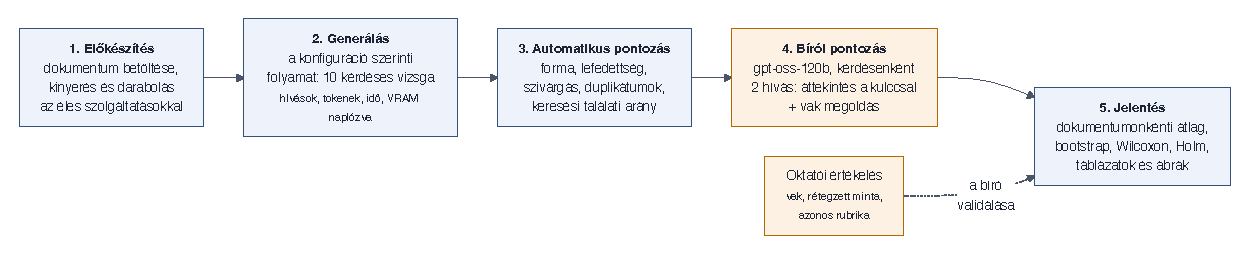
\includegraphics[width=0.9\textwidth]{figures/d4_kiertekeles}
\caption[Egy teszt lépései.]{Egy teszt lépései: előkészítés a szolgáltatásokon, generálás a konfiguráció szerint,
automatikus mutatók, bírói pontozás és összesítés.}
\label{fig:kiertekeles}
\end{figure}

A reprodukálhatóságot négy mechanizmus biztosítja: (1) minden futás rögzíti a teljes konfigurációt, a kód
és az adatkészlet verzióját és a hardvert; (2) a bíró válaszai lemezre, gyorsítótárba kerülnek, a bírómodell,
a promptverzió, a gondolkodási szint és a teljes prompt kivonatával mint kulccsal, így újrapontozáskor
ugyanarra a kérdésre ugyanaz az ítélet jön, és egy mutató utólagos módosítása nem igényel bírói hívást;
(3) a \code{-{}-resume} kapcsoló csak a hiányzó vagy sikertelen vizsgákat futtatja újra; (4) a
keretrendszert 43 automatikus teszt fedi le, köztük ál-szolgáltatásokkal és ál-nyelvi modellel a teljes
folyamat.

% ---------------------------------------------------------------------
\section{Adatkészlet}
\label{sec:adatkeszlet}
% ---------------------------------------------------------------------

Az \code{eval-v1} adatkészlet 39 dokumentumból áll (\ref{tab:adatkeszlet}.~táblázat,
\ref{app-adatkeszlet}.~függelék): három saját, rövid magyar oktatási szöveg (kávé, immunrendszer,
játékelmélet) kézzel írt referenciakérdésekkel, 12 OpenStax-tankönyvrészlet az EduQG~\cite{hadifar2023eduqg}
szakértői kérdéseivel és 24 magyar Wikipédia-cikk a MILQA~\cite{novak2023milqa} szövegértési kérdéseivel,
összesen 326 referenciakérdéssel. A fő vizsgálat ebből 30-at használt: mind a 24 MILQA-cikket, a 3 saját
szöveget és 3 OpenStax-részletet (\code{en-economics-short-01}, \code{en-humanities-medium-02},
\code{en-law-long-03}), összesen 27 magyar és 3 angol dokumentumot, hosszúság szerint 12 rövid, 9 közepes
és 9 hosszú dokumentummal. A szűkítés oka a futásidő volt; az elsődleges cél a magyar nyelvű kiértékelés,
az angol részletek a nyelvi összevetést szolgálják. A referenciakérdések \emph{nem} célok, hiszen egy jó
vizsgakérdésnek nem kell hozzájuk hasonlítania; a keresés pontosságát és a tematikus egyezést mérjük velük.

% ---------------------------------------------------------------------
\section{A kísérleti konfigurációk}
\label{sec:karok}
% ---------------------------------------------------------------------

A kísérleti terv \emph{egytényezős}: minden konfiguráció egy referenciakonfigurációhoz képest pontosan
egy tényezőben tér el, így a kettő különbsége az adott tényezőnek tulajdonítható.
\Az{\ref{tab:karok}}.~táblázat a 14 konfigurációt három csoportban
foglalja össze.

\begin{table}[htbp]
\centering
\caption[A kísérleti konfigurációk.]{A kísérleti konfigurációk. Ref.: amelytől a konfiguráció egyetlen tényezőben eltér; Magok:
dokumentumonkénti ismétlések száma az előzetes és a fő vizsgálatban (a pilotban mindenhol 3);
Vizsg.: P = pilot, Ev = előzetes vizsgálat, F = fő vizsgálat.}
\label{tab:karok}
\small
\begin{tabularx}{\textwidth}{@{}l>{\raggedright\arraybackslash}Xccl@{}}
\toprule
Jel & Mit változtat & Ref. & Magok & Vizsg. \\
\midrule
\multicolumn{5}{@{}l}{\emph{Alapvonalak}} \\
\arm{B-doc-L} & teljes dokumentum egy promptban, helyi modell ($\le$\,30\,000 karakter) & -- & 3 & Ev, F \\
\arm{B-doc-S} & ugyanez a szervermodellel ($\le$\,80\,000 karakter) & -- & 3 & Ev \\
\arm{E0}  & naiv RAG: a kéréshez legközelebbi 3 darab, a vizsga egy hívásban & -- & 3 & P, Ev, F \\
\midrule
\multicolumn{5}{@{}l}{\emph{A módszer lépései}} \\
\arm{E1}  & vizsgaterv, kérdéshelyenkénti keresés és generálás, ellenőrzés nélkül & \arm{E0} & 1 & P, Ev, F \\
\arm{E2}  & \arm{E1} + ellenőrző lánc visszacsatolással (a teljes módszer) & \arm{E1} & 1 & P, Ev, F \\
\arm{E3}  & \arm{E2} + fogalomgráf & \arm{E2} & 1 & P, Ev, F \\
\midrule
\multicolumn{5}{@{}l}{\emph{Kiegészítő ablációk}} \\
\arm{E2f} & \arm{E2} vak megoldási próba nélkül & \arm{E2} & 1 & P, Ev, F \\
\arm{E2h} & \arm{E2} hibrid (BM25 + sűrű) kereséssel & \arm{E2} & 1 & P, Ev, F \\
\arm{E2x} & \arm{E2}, az ellenőrzést egy másik modell (Llama-3.1-8B) végzi & \arm{E2} & 1 & Ev, F \\
\arm{E4}  & \arm{E0} a szervermodellel & \arm{E0} & 3 & P, Ev \\
\arm{E4b} & \arm{E2} a szervermodellel & \arm{E2} & 1 & Ev \\
\arm{E5a} & \arm{E0} a régi, 512 tokenre csonkolt kódolóval & \arm{E0} & 3 & P, Ev, F \\
\arm{E5b} & \arm{E0}, vágási küszöb: átlag $+\,1{,}5$ szórás & \arm{E0} & 3 & P, Ev, F \\
\arm{E5c} & \arm{E0} rögzített, 800 karakteres darabokkal & \arm{E0} & 3 & P, Ev, F \\
\bottomrule
\end{tabularx}
\end{table}

Az \emph{alapvonalak} azt modellezik, amit egy oktató a \Mimir{} nélkül tenne: a \arm{B-doc-S} a mai
gyakorlat (a jegyzet feltöltése egy csevegő asszisztensbe), a \arm{B-doc-L} ugyanez a helyi modellel,
16\,384 tokenes kontextussal, az \arm{E0} a rendszer mai működése. Az \arm{E1}--\arm{E0} különbség a
tervezés (\ref{h:terv}.~és \ref{h:lefed}.~hipotézis), az \arm{E2}--\arm{E1} az ellenőrzés
(\ref{h:verif}.~hipotézis), az \arm{E3}--\arm{E2} a fogalomgráf hatása; az \arm{E2}-ben az ellenőrzést a
kérdést író modell végzi. Az \arm{E2x} ellenőrzője a PULI-LlumiX esetében a generátor alapmodellje, tehát
nem független család; az \arm{E4} és az \arm{E4b} a \ref{h:helyi}.~hipotézist, az \arm{E5a}--\arm{E5c} a
darabolás hatását vizsgálja (régi kódoló: \ref{sec:csonkolt}.~szakasz; rögzített
darabolás~\cite{qu2024chunking}). A konfigurációk egytényezős fáját
\az{\ref{fig:kiserleti-terv}}.~ábra (\ref{app-karok}.~függelék) mutatja.

A tervezett konfigurációk egy maggal futnak, mert egy vizsga perceket igényel, és a variancia fő forrása
a dokumentum; az olcsó egyhívásos konfigurációk zaját három mag csökkenti. A tervben szereplő \arm{E0s}
(az \arm{E0} az éles végponton át) egyik vizsgálatban sem futott. Előre rögzített, a többszörös
összehasonlítás korrekciójába tartozó páros összehasonlítás hat van: \arm{E1}--\arm{E0}
(tervezés), \arm{E2}--\arm{E1} (ellenőrzés), \arm{E2}--\arm{E0} (teljes módszer), \arm{E2}--\arm{B-doc-L}
(módszer vs.\ teljes dokumentumos prompt), \arm{E2x}--\arm{E2} (ellenőrző modell) és \arm{E3}--\arm{E2}
(gráf); a többi összevetés leíró jellegű.

% ---------------------------------------------------------------------
\section{A három vizsgálat}
\label{sec:vizsgalatok}
% ---------------------------------------------------------------------

A kísérleteket három lépcsőben futtattuk (\ref{tab:vizsgalatok}.~táblázat). A \emph{pilot} a mérési
láncot próbálta ki; egy dokumentumon hipotézist eldönteni elvileg sem lehet. Az \emph{előzetes vizsgálat} a
pilot után javított folyamattal (szivárgási szabályok, javító hívás, $r=1$, a bíró a kérdés forrásdarabjait
kapja), a \emph{fő vizsgálat} ugyanezzel, 30 dokumentumon és két helyi generátorral futott.

\begin{table}[htbp]
\centering
\caption[A három vizsgálat beállításai.]{A három vizsgálat beállításai. Pontozott kérdés: a generált
vizsgákból pontozásra került kérdés; a bírói áttekintő ítélet ezek egy részénél hiányzik.}
\label{tab:vizsgalatok}
\small
\begin{tabularx}{\textwidth}{@{}>{\raggedright\arraybackslash}p{2.6cm}>{\raggedright\arraybackslash}p{3.1cm}>{\raggedright\arraybackslash}X>{\raggedright\arraybackslash}X@{}}
\toprule
 & Pilot & Előzetes vizsgálat & Fő vizsgálat \\
\midrule
Időpont (2026) & szept.\ 23. & szept.\ 27--28. & okt.\ 7.\ -- nov.\ 1. \\
Dokumentumok & 1 (\code{hu-coffee}, 1\,702 karakter) & 9 (3 saját magyar, 6 angol); konfigurációnként 6 & 30 (24 MILQA, 3 saját, 3 OpenStax) \\
Konfigurációk & 10 & 14 & 11 helyi, mindkét generátorral \\
Generátor & Qwen2.5-7B (\arm{E4}: szervermodell) & Qwen2.5-7B; szervermodell (\arm{B-doc-S}, \arm{E4}, \arm{E4b}) & PULI-LlumiX 8B és Gemma 3 12B \\
Ismétlés & 3 mag mindenhol & 3 mag (egyhívásos konfigurációk), 1 mag (tervezett konfigurációk) & mint az előzetes vizsgálatban \\
Pontozott kérdések & 300 & 1\,670 (mindegyik bírói áttekintő ítélettel) & PULI: 2\,935; Gemma: 6\,212; bírói áttekintő ítélet a kérdések 29--65\,\%-ánál (a PULI egyhívásos konfigurációinál 70--100\,\%-ánál), lásd \ref{sec:fo-meres}.~szakasz \\
Újrapróbálkozás ($r$) & 2 & 1 & 1 \\
Szivárgási szabály, javító hívás & nincs & van & van \\
Bíró forrása & a teljes dokumentum & a kérdés forrásdarabjai (teljes dokumentumos konfigurációknál a dokumentum első 24\,000 karaktere) & mint az előzetes vizsgálatban \\
GPU & RTX 3070 Ti (8\,GiB), asztali PC & RTX A4500 (20\,GiB), egyetemi munkaállomás & RTX A4500 (20\,GiB), egyetemi munkaállomás \\
\bottomrule
\end{tabularx}
\end{table}

Az előzetes vizsgálatban az \arm{E4} és az \arm{E4b} hat angol dokumentumon futott (ebből három közös), a
többi konfiguráció a közös hat dokumentumon. A PULI-LlumiX-nél azért kevesebb a pontozott kérdés, mert
gyakran tíznél kevesebb kérdést adott vissza. A 20\,GiB-os munkaállomás-kártyán a modell, a kvantálás és a
kontextus ugyanaz, mint egy fogyasztói kártyán, így ez a minőséget nem befolyásolja, a memóriamérés pedig a
modell saját foglalását adja.

\paragraph{Két összevetési szabály.} A vizsgálatok eltérő dokumentumokon, generátorokkal és részben eltérő
implementációval futottak, ezért az eredményeket két szabály szerint vetjük össze.
\begin{enumerate}[label=(\arabic*)]
\item \emph{Összevetés csak azonos dokumentumokon.} Két konfigurációt, két modellt vagy két vizsgálatot
csak ugyanazon a dokumentumhalmazon hasonlítunk össze, mert a variancia fő forrása a dokumentum
(\ref{sec:statisztika}.~szakasz). Egy vizsgálaton belül ez a közös dokumentumokon teljesül. A három
vizsgálat között az összevetés a \emph{hat közös dokumentumon} megengedett (a három saját magyar szöveg és
a fő vizsgálat három OpenStax-részlete), amelyen az előzetes vizsgálat Qwen2.5-7B-je és a fő vizsgálat két
modellje egyaránt futott; ilyenkor ezt mindig jelezzük. A pilot az akkori, javítás előtti folyamatot méri,
ezért vele számszerű összevetést nem végzünk.
\item \emph{A futásidő relatív szorzó.} A futásidőt azzal mérjük, hogy ugyanazon a GPU-n egy konfiguráció
hányszor lassabb a referenciánál (például az \arm{E2} az \arm{E0}-nál). Mivel a döntéshez a módszerek
egymáshoz mért aránya kell, a GPU típusa ezt érdemben nem befolyásolja; az abszolút perceket csak
mellékesen közöljük. A pilot RTX 3070 Ti-n, az előzetes és a fő vizsgálat RTX A4500-on futott, ezért a
szorzókat is mindig egy vizsgálaton belül számoljuk (\ref{sec:fo-koltseg}.~szakasz).
\end{enumerate}

% ---------------------------------------------------------------------
\section{Mutatók}
\label{sec:mutatok}
% ---------------------------------------------------------------------

Minden ráta 0 és 1 (0 és 100\,\%) közötti, és a szivárgás, a nem kérdő törzs és a duplikátumok
kivételével a nagyobb érték a jobb. A tartalmi mutatók a bíró ítéletén alapulnak. Az
\emph{alátámasztottság} ($G$) azon kérdések aránya, amelyeknél a forrás igazolja a megjelölt kulcsot (a
bírónak az igazoló mondatot szó szerint idéznie kell); a \emph{vak megoldhatóság} ($A$) azoké, amelyeket a
bíró a kulcs ismerete nélkül, összekevert válaszokkal, csak a forrás alapján helyesen old meg -- ez a kulcs
helyességét és a kérdés egyértelműségét együtt méri; a \emph{disztraktor-validitás} ($V$) a kérdésenkénti
azon disztraktorok aránya, amelyek a forrás szerint hamisak \emph{és} témába vágók. A \emph{formai
megfelelés} ($F$) vizsgaszintű igen/nem érték: a vizsga pontosan a kért számú kérdést tartalmazza, és
minden kérdésnek pontosan négy válasza és egy kulcsa van. A négyet egy \emph{minőségi indexbe} foglaljuk:
\begin{equation}
Q=\frac{F+G+A+V}{4}.
\label{eq:qindex}
\end{equation}
A $Q$ szándékosan egyszerű, súlyozatlan átlag, amelyet vizsgánként számolunk; a sikertelen vizsga
(értelmezhetetlen modellválasz) $Q$-ja 0, a technikai (szolgáltatás-) hibák kimaradnak. Egyetlen hibás
formájú vagy hiányzó kérdés így a $Q$-t $0{,}25$-tel csökkenti; ezt vállaljuk, mert egy hiányos vagy hibás
kulcsú vizsga nem használható változtatás nélkül. A komponenseket külön is közöljük.

A bíró emellett négy szempontot 1--5 skálán pontoz (\emph{helyesség}, \emph{érthetőség},
\emph{disztraktorok}, \emph{szintillesztés}), és igen/nem ítéletet ad (\emph{felhasználnám}: bekerülne-e
egy valódi dolgozatba legfeljebb apró javítással). A rubrika (\ref{app-rubrika}.~függelék) a bíró és az
oktatók számára azonos, ami a bíró validálásának (\ref{h:meres}.~hipotézis) előfeltétele. A
\emph{lefedettség} (\ref{eq:cov}.~egyenlet) a kérdésekhez legközelebbi különböző darabok aránya a
dokumentum darabjai között (a P2 probléma mérőszáma); mivel tíz kérdésnél legfeljebb $10/K$ ($K$ a
darabszám), csak azonos dokumentumon, konfigurációk között hasonlítható, és szerkezeti mutatóként a $Q$-ba
nem számít bele. A \emph{szivárgást} és a \emph{nem kérdő törzset} ugyanazzal a szabállyal mérjük, mint az
ellenőrző (\ref{sec:verifier}.~szakasz; vö.\ \ref{sec:szivargas}.~szakasz). A duplikátumráta, a
meta-hivatkozás, a keresési találati arány (recall@3), a tematikus hasonlóság és a költségmutatók
definíciója \az{\ref{app-mutatok}}.~függelékben található.

% ---------------------------------------------------------------------
\section{A bíró}
\label{sec:biro}
% ---------------------------------------------------------------------

A bíró a gpt-oss-120b~\cite{gptoss2025} modell az egyetemi GenAI-szerveren, nulla hőmérséklettel és
alacsony („low”) gondolkodási szinttel. Más modellcsaládba tartozik, mint bármelyik generátor (Qwen,
Llama/PULI, Gemma), ami az önpreferencia torzításának~\cite{panickssery2024selfpref} kockázatát
csökkenti. Kérdésenként két hívást végez: az \emph{áttekintő} hívás látja a kulcsot (alátámasztottság szó
szerinti idézettel, disztraktoronkénti ítélet, rubrikapontok, megvalósult Bloom-szint, „felhasználnám”), a
\emph{vak} hívás nem, és permutált válaszokkal kell megoldania a kérdést.

Forrásként a bíró a kérdéshez tartozó darabokat kapja (a tervezett konfigurációknál a kérdéshely
kontextusát, az \arm{E0}-nál a visszakeresett darabokat), a megosztott szerver futásideje miatt nem a
teljes dokumentumot; így a dokumentum más részeiben lévő ellentmondást nem látja. A teljes dokumentumos
konfigurációknál a dokumentum első 24\,000 karakterét kapja, ezért ott az alátámasztottság alsó becslés. A
fő vizsgálatban a bíró szervere a kérések egy részére hibával válaszolt; a hiányzó áttekintő ítéletek
aránya forrásonként és modellenként eltér (\ref{tab:vizsgalatok}.~táblázat), a bírón alapuló mutatók csak
az ítélettel rendelkező kérdésekre számolódnak, a hatást és egy érzékenységvizsgálatot
\az{\ref{sec:fo-meres}}.~szakasz mutatja be.

% ---------------------------------------------------------------------
\section{Oktatói értékelés}
\label{sec:oktatoi}
% ---------------------------------------------------------------------

A bíró csak akkor érvényes mérőeszköz, ha ítéletei az emberi szakértőkével egyeznek
(\ref{h:meres}.~hipotézis). Az oktatói értékelés a dolgozat lezárásakor folyamatban van; protokollját a
keretrendszer \code{rate-export} és \code{rate-import} lépése valósítja meg: konfigurációnként 30 vakon
értékelt kérdés, 3 értékelő, a bíróéval azonos rubrika és forrásrészlet; az egyezést
Krippendorff-$\alpha$-val~\cite{krippendorff2004}, Spearman-korrelációval és Cohen-$\kappa$-val mérjük
(részletek: \ref{app-oktatoi}.~függelék). Az eredményeket \az{\ref{sec:oktatoi-eredmeny}}.~szakasz közli.

% ---------------------------------------------------------------------
\section{Statisztikai elemzés}
\label{sec:statisztika}
% ---------------------------------------------------------------------

\paragraph{Az elemzés egysége a dokumentum.} Egy vizsga tíz kérdése nem független: ugyanabból a
dokumentumból, egy futáson belül készül, így független megfigyelésként kezelve a próbák a valósnál
biztosabbnak mutatnák az eredményt. Ezért minden mutatót előbb dokumentumon belül átlagolunk (a kérdésekre
és a magokra); a konfigurációnkénti érték a dokumentumonkénti átlagok átlaga. Bizonytalanságát
\emph{bootstrap}-módszerrel~\cite{efron1993} becsüljük: a dokumentumokból 10\,000-szer húzunk
visszatevéssel, és a kapott átlagok középső 95\,\%-a adja a 95\,\%-os konfidenciaintervallumot.

\paragraph{Páros összehasonlítás és többszörös tesztelés.} Két konfigurációt a páros Wilcoxon-féle
előjeles rangpróbával~\cite{wilcoxon1945} vetünk össze, amely a dokumentumonkénti különbségek rangjaival
dolgozik, és nem feltételez normális eloszlást (ez a plafonhoz közeli rátáknál lényeges); a hatás nagysága
a rangbiszeriális korreláció~\cite{kerby2014} (\ref{eq:rrb}.~egyenlet, \ref{app-statisztika}.~függelék),
amely $+1$, ha az új konfiguráció minden dokumentumon jobb, és $-1$, ha mindenütt rosszabb. A hat előre
rögzített összehasonlítás $p$-értékeit Holm módszerével~\cite{holm1979} korrigáljuk: növekvő sorrendben a
legkisebbet 6-tal, a következőt 5-tel stb.\ szorozzuk, és egy összevetés csak akkor szignifikáns, ha
korrigált értéke (és minden nála kisebbé) $0{,}05$ alatt van. A Wilcoxon-próba legkisebb elérhető
$p$-értéke hat dokumentumnál $0{,}031$, korrekció után $0{,}19$ (levezetés: \ref{app-statisztika}.~függelék):
a pilot ezért csak leíró, az előzetes vizsgálatban egyetlen összevetés sem lehet korrekció után
szignifikáns, a fő vizsgálat 30 dokumentumán viszont a szignifikancia elérhető.

\paragraph{Egyezés és az ellenőrző mint osztályozó.} Két igen/nem ítéletsor (például az ellenőrzőé és a
bíróé) egyezését Cohen-$\kappa$-val~\cite{cohen1960kappa} mérjük (\ref{eq:kappa}.~egyenlet; $\kappa=0$ a
véletlen szintje, $\kappa=1$ a teljes egyezés, az értelmezés Landis és Koch~\cite{landis1977} skáláját
követi). Az ellenőrző minden kérdést \emph{átengedett} vagy \emph{megjelölt} kategóriába sorol; a bíró
alátámasztottsági ítéletét referenciának tekintve pontosságot és felidézést számolunk
(\ref{eq:precrec}.~egyenlet). Hasznos ellenőrzőtől mindkettő magas értéke és $\kappa\gg0$ várható;
$\kappa\approx0$ esetén a jelzése az oktatónak nem hordoz információt.

\bigskip
\noindent\textbf{A fejezet tanulsága.} A kiértékelés nem egy szám, hanem egy mérési lánc: egytényezős
konfigurációk, a forráshoz mért mutatók, egy független, de maga is ellenőrzött bíró és a dokumentumot
egységnek tekintő statisztika együtt teszik lehetővé, hogy egy különbséget egyetlen tényezőnek
tulajdonítsunk, és lássuk, mikor nem szignifikáns. A két összevetési szabály a vizsgálatok eltérő
dokumentumaiból és hardveréből adódó torzítást zárja ki. A következő két fejezet ezzel a lánccal értékeli
előbb a módszer lépéseit (\ref{ch:eredmenyek}.~fejezet), majd a modelleket (\ref{ch:modellek}.~fejezet).
